% PREAMBLE
%%%%%%%%%%
%%%%%%%%%%

\documentclass[oneside,a4paper]{scrartcl}

% PACKAGES
%%%%%%%%%%
\usepackage[english]{babel}
\usepackage{graphicx}
\usepackage{pgf}
\usepackage{placeins}
\usepackage{listings}


% DOCUMENT
%%%%%%%%%%
%%%%%%%%%%

\begin{document}

%%%%%%%
% TITLE
%%%%%%%

\title{Exercise Sheet VII}
\subject{Advanced Parallel Computing}
\author{Klaus Naumann \& Christoph Klein}
\maketitle

%%%%%%%
% PART 1 - Reading
%%%%%%%
\section{Review: Why The Grass May Not Be Greener On The Other Side: A Comparison of Locking vs Transactional Memory}
In their paper McKeeney et al. examined and compared the benefits and disadvantages of 
locking and transactional memory. The authors analyzed scope, composability, scalability, 
performance, hardware / software support and a possible symbiosis with other synchronization 
mechanisms.
\\
McKeeney et al. outline that combining the benefits of different synchronization methods 
could be the best way to go. This approach will possibly enable an high exploit of a multi-core 
systems performance potential. TM has benefits compared to locking but is in a too early 
state to make clear claims about its interaction with other mechanisms.
\\
To our mind an interaction between various synchronization mechanism could be a 
performance-boost for application with artifacts in need for different synchronization strategies. 
Further investigation should deal with TM supporting hardware and possibilities to make TM 
usable in terms of programming models.
     
\section{Review: Stretching Transactional Memory}
In their June 2009 released paper \emph{Stretching Transactional Memory} Dragojevic et al. 
propose a new software transactional memory called SwissTM. SwissTM - lock- and 
word-based - supports an optimistic (read/write) and a pessimistic (write/write) conflict 
detection and a two-phase contention manager avoiding overhead on short transactions while 
ensuring the progress of long ones.
\\
The authors outline that SwissTM outperforms state-of-the-art STMs in workloads dominated by 
non-uniform, dynamic data structures, non-static transaction sizes and mixed access patterns. 
Additionaly SwissTMs performs well for workloads with a smaller scale. To further optimize the 
performance of SwissTM the authors suggest improving the programming model by adding compiler 
support and making SwissTM privatization-safe.
\\
To our mind SwissTM is a step in the right direction to adopt STM in commercial applications 
like business software. As the authors mentioned it is necessary to improve the programming model 
to make SwissTM more \emph{usable}.
  

%%%%%%%
% PART 2 - Experiments
%%%%%%%

\section{Red-Black Tree -- Experiments}
We executed the program with a ration of 90/10 (Search operations / Add operations).
\\
\begin{center}
\begin{tabular}{l|l}
Operations & Operations per Second\\\hline
100k & 417.573 \\
500k & 413.259\\
1M & 470.808\\
5M & 429.344\\
10M & 397848\\
25M & 446.870\\
50M & 464820\\
\end{tabular}
\end{center}\\
\\
\\
As you can see with increasing operations the results of our experiment are on a relatively constant and high level. The reason for this is the structure of a red-black tree. It allows searching and inserting operations in O(\log{n}).
\\
\begin{center}
	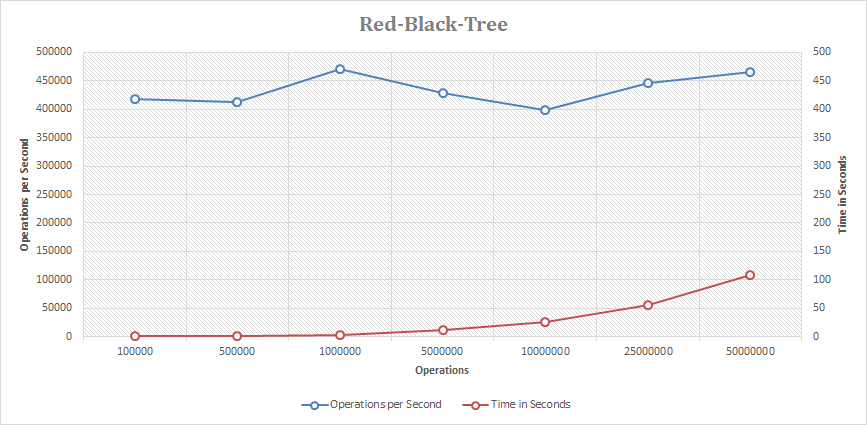
\includegraphics[width=0.8\columnwidth]{results.png}\\
	\caption{Sequential Red-Black Tree execution with a ratio of 90/10 (Search operations / Add operations) 
	on \emph{moore}. Results are represented as \it{Operations/seconds}.}
\end{center}
\\\\
\\\\
\end{document}
